\testfile{pgfplotstest.colormap.tex}
{
\testsection{Basic level experiment}
Experiment:
\begin{itemize}
	\item Define a color map,
	\item convert it back to a shading; draw that shading,
	\item for a set of sample points, map them linearly into the color map and draw small ``tick'' lines over the shading.
\end{itemize}

The test PASSES IF AND ONLY IF: the shading and the ``tick'' lines have the same color.

Color spec: {rgb(0cm)=(1,0,0); rgb(2cm)=(0,0.5,0);  gray(4cm)=(0.2);  color(6cm)=(green); }

\pgfplotscreatecolormap{my map}{rgb(0cm)=(1,0,0); rgb(2cm)=(0,0.5,0);  gray(4cm)=(0.2);  color(6cm)=(green); }

\def\LENGTH{300}

\pgfplotscolormaptoshadingspec{my map}{\LENGTH pt}\temp
\def\tempb{\pgfdeclarehorizontalshading{myshadingA}{1cm}}
\expandafter\tempb\expandafter{\temp}

\begin{tikzpicture}
	\draw (0pt,0pt) rectangle (\LENGTH pt,3cm);
	\pgftext[left,bottom,at=\pgfpoint{0pt}{0pt}]{\pgfuseshading{myshadingA}}%
	\foreach \i in {0,10,...,\LENGTH .001} {
		\pgfplotscolormapfind[0:\LENGTH]{\i}{my map}%
		\def\tempb{\definecolor{tempcolor}{rgb}}
		\expandafter\tempb\expandafter{\pgfmathresult}
		\fill[tempcolor] (\i pt,1cm) rectangle (\i pt + 2pt,2cm);
	}
\end{tikzpicture}

\testsection{Colorbars}
\testsubsection{default config}
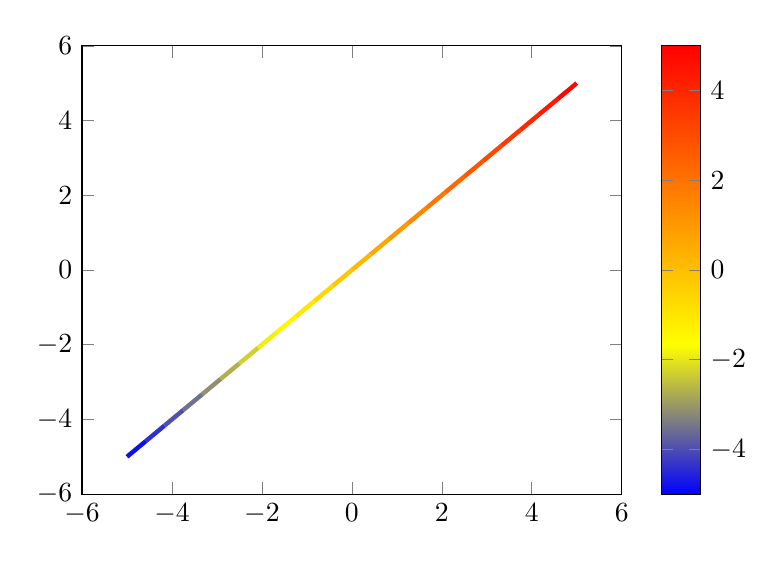
\begin{tikzpicture}
	\begin{axis}[colorbar]
		\addplot[mesh,ultra thick] {x};
	\end{axis}
\end{tikzpicture}

\testsubsection{colorbar right}
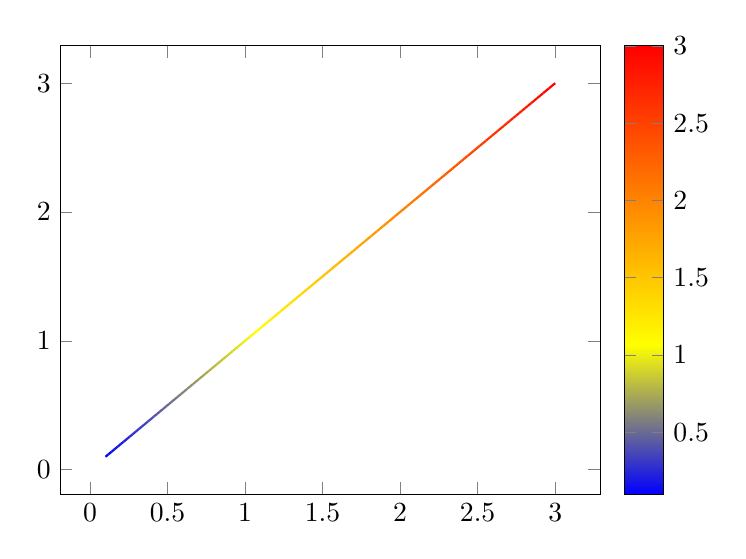
\begin{tikzpicture}
	\begin{axis}[colorbar right]
	\addplot[mesh,thick,samples=150,domain=0.1:3] 
		{x};
	\end{axis}
\end{tikzpicture}

\testsubsection{colorbar left}
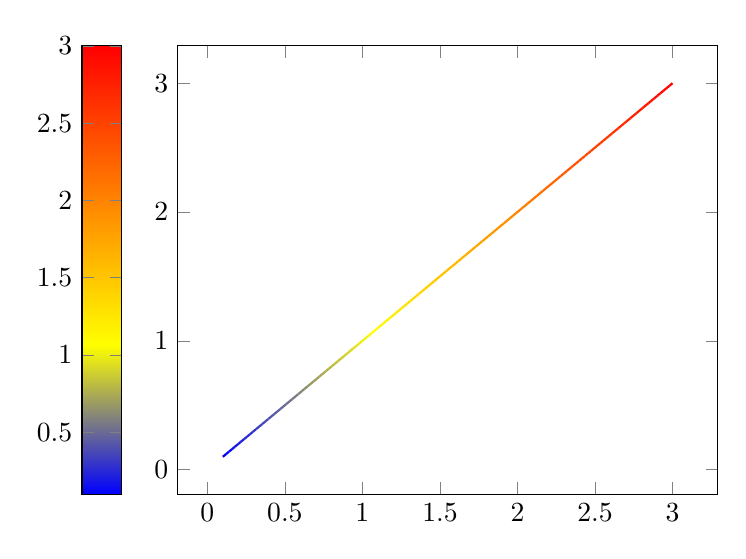
\begin{tikzpicture}
	\begin{axis}[colorbar left]
	\addplot[mesh,thick,samples=150,domain=0.1:3] 
		{x};
	\end{axis}
\end{tikzpicture}

\testsubsection{colorbar horizontal}
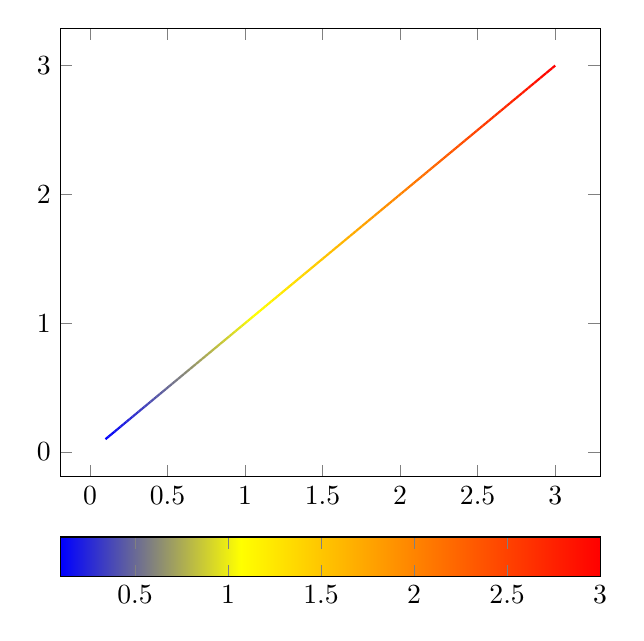
\begin{tikzpicture}
	\begin{axis}[colorbar horizontal]
	\addplot[mesh,thick,samples=150,domain=0.1:3] 
		{x};
	\end{axis}
\end{tikzpicture}

\testsubsection{colorbar horizontal; top with customization}
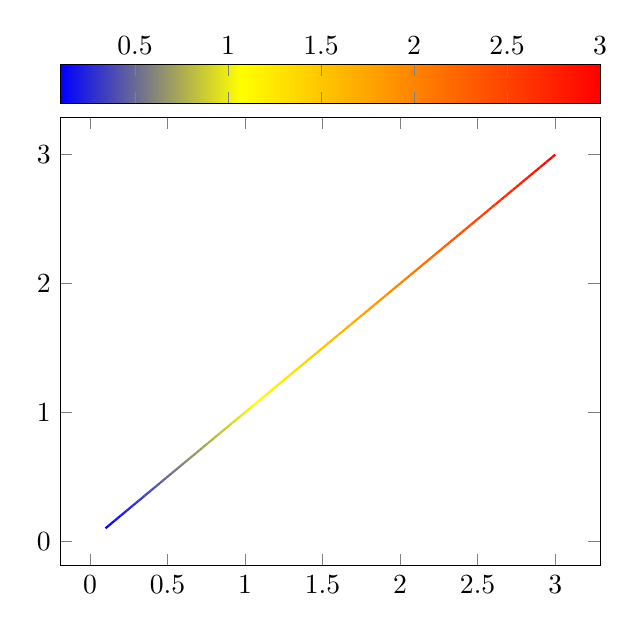
\begin{tikzpicture}
	\begin{axis}[colorbar horizontal, colorbar style={at={(0.5,1.03)},anchor=south,xticklabel pos=right}]
	\addplot[mesh,thick,samples=150,domain=0.1:3] 
		{x};
	\end{axis}
\end{tikzpicture}

\testsubsection{colorbar horizontal; top with even more customization}
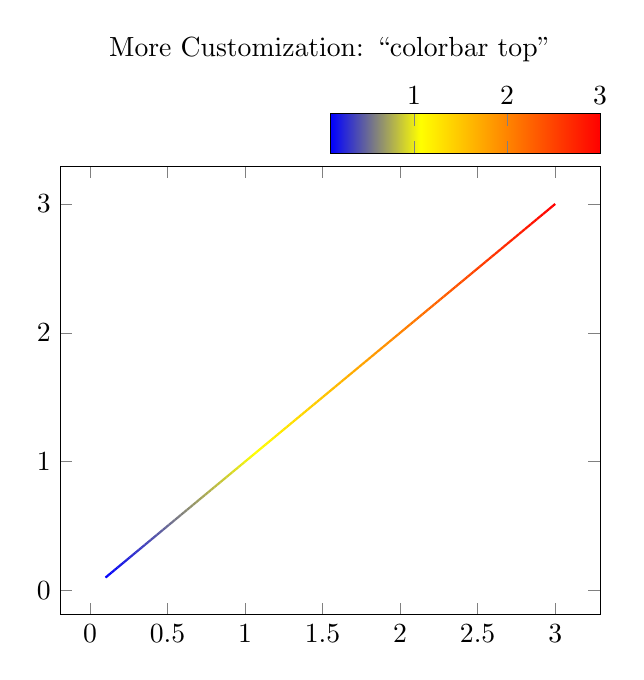
\begin{tikzpicture}
	\begin{axis}[colorbar horizontal, colorbar style={at={(1,1.03)},anchor=south east,width=0.5*\pgfkeysvalueof{/pgfplots/parent axis width},xticklabel pos=right},
	title style={yshift=1cm},
	title=More Customization: ``colorbar top'',
	]
	\addplot[mesh,thick,samples=150,domain=0.1:3] 
		{x};
	\end{axis}
\end{tikzpicture}

\testsubsection{Testing at=(1.03,0.5),anchor=west}
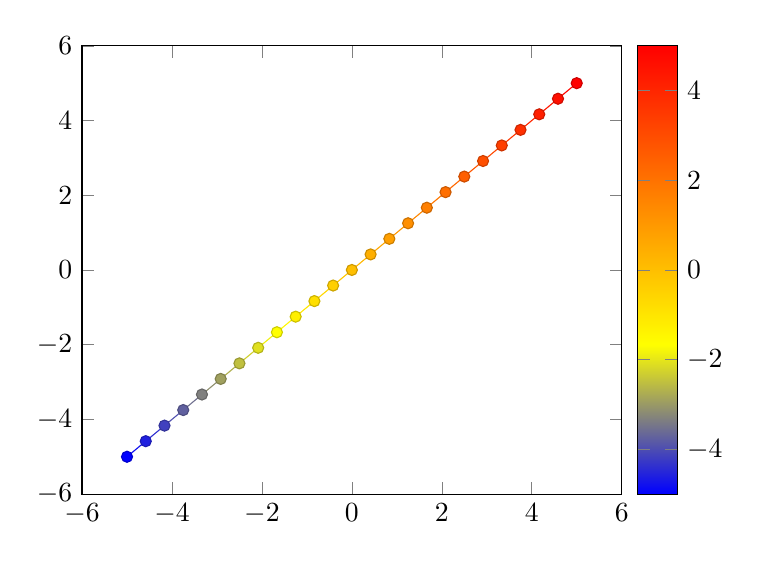
\begin{tikzpicture}
	\begin{axis}[colorbar,colorbar style={at={(1.03,0.5)}, anchor=west},colorbar shift/.style={}]
		\addplot+[mesh,scatter] {x};
	\end{axis}
\end{tikzpicture}
}
